% !TEX root = saveliev_physics_general_course_2.tex
%!TEX TS-program = pdflatex
%!TEX encoding = UTF-8 Unicode


\chapter[OPTICS]{OPTICS}\label{chap:16}
\chaptermark{OPTICS}

\section{The Light Wave}\label{sec:16_1}

Light is a complicated phenomenon: in some cases it behaves like an electromagnetic wave, in others like a stream of special particles (photons).
In the present volume, we shall treat wave optics, \ie, the range of phenomena based on the wave nature of light.
The collection of phenomena due to the corpuscular (particulate) nature of light will be dealt with in Volume III.

What oscillates in an electromagnetic wave are the vectors $\vec{E}$ and $\vec{H}$.
Experiments show that the physiological, photochemical, photoelectrical and other actions of light are due to the oscillations of the electric vector.
Accordingly, we shall speak in the following of the \textbf{light vector}, having in mind the electric field strength vector.
We shall meanwhile make no mention of the magnetic vector of a light wave.

We shall designate the magnitude of the light vector amplitude, as a rule, by the letter $A$ (sometimes by the symbol $\ab{E}{m}$).
Hence, the change in space and time of the projection of the light vector onto the direction along which it oscillates will be described by the equation
\begin{equation}\label{eq:16_1}
    E = A \cos(\omega t - kr + \alpha),
\end{equation}

\noindent
where $k$ is the wave number and $r$ is the distance measured along the direction of propagation of the light wave.

For a plane wave propagating in a non-absorbing medium, $A = \text{constant}$, for a spherical wave, $A$ diminishes in proportion to $1/r$, and so on.

The ratio of the speed of a light wave in a vacuum to the phase velocity $v$ in a medium is known as the \textbf{absolute refractive index} of the medium and is designated by the letter $n$.
Thus,
\begin{equation}\label{eq:16_2}
    n = \frac{c}{v}.
\end{equation}

\noindent
A comparison with \eqn{15_10} shows that $n = \sqrt{\varepsilon\mu}$.
For the overwhelming majority of transparent substances, $\mu$ does not virtually differ from unity.
We can therefore consider that
\begin{equation}\label{eq:16_3}
    n = \sqrt{\varepsilon}.
\end{equation}

Equation \eqref{eq:16_3} relates the optical and the electrical properties of a substance.
It may seem on the face of it that this equation is wrong.
For example, for water $\varepsilon = 81$, whereas $n = 1.33$.
It must be borne in mind, however, that the value $\varepsilon = 81$ has been obtained from electrostatic measurements.
A different value of $\varepsilon$ is obtained for fast-varying electric fields, and it depends on the frequency of oscillations of the field.
This explains the \textbf{dispersion} of light, \ie, the dependence of the refractive index (or speed of light) on the frequency (or wavelength).
Using the value of $\varepsilon$ obtained for the relevant frequency in \eqn{16_3} leads to the correct value of $n$.

The values of the refractive index characterize the \textbf{optical density} of the medium.
A medium with a greater $n$ is called optically denser than one with a smaller $n$.
Conversely, a medium with a lower $n$ is called optically less dense than one with a greater $n$.

The wavelengths of visible light are within the following limits:
\begin{equation}\label{eq:16_4}
    \lambda_0 = \text{\SIrange{0.40}{0.76}{\micro\metre}} (\text{\SIrange{4000}{7600}{\angstrom}}).
\end{equation}

\noindent
These values relate to light waves in a vacuum.
The lengths of light waves in substances will have other values.
For oscillations of frequency $\nu$, the wavelength in a vacuum is $\lambda_0 = c/\nu$.
In a medium in which the phase velocity of a light wave is $v = c/n$, the wavelength has the value $\lambda = v/\nu = c/(\nu n) = \lambda_0/n$.
Thus, the length of a light wave in a medium with the refractive index $n$ is related to the wavelength in a vacuum by the expression
\begin{equation}\label{eq:16_5}
    \lambda = \frac{\lambda_0}{n}.
\end{equation}

The frequencies of visible light waves are within the limits
\begin{equation}\label{eq:16_6}
    \nu = \text{\SIrange{0.39e15}{0.75e15}{\hertz}}.
\end{equation}

\noindent
The frequency of the changes in the vector of the energy flux density carried by a wave will be still greater (it equals $2\nu$).
Neither our eye nor any other receiver of luminous energy can track such frequent changes in the energy flux, hence, they register the time-averaged flux. The magnitude of the time-averaged energy flux density carried by a light wave is called the \textbf{light intensity} $I$ at the given point of space.
The density of the flux of electromagnetic energy is determined by the Poynting vector $\vec{S}$.
Hence,
\begin{equation}\label{eq:16_7}
    I = |\average{\vec{S}}| = |\average{\vecprod{E}{H}}|.
\end{equation}

\noindent
Averaging is performed over the time of ``operation'' of the instrument, which, as we have already noted, is much greater than the period of oscillations of the wave.
The intensity is measured either in energy units (for example, in \si{\watt\per\metre\squared}), or in light units named ``lumen per square metre'' (see \sect{16_5}).

According to \eqn{15_22}, the magnitudes of the amplitudes of the vectors $\vec{E}$ and $\vec{H}$ in an electromagnetic wave are related by the expression
\begin{equation*}
    \ab{E}{m} \sqrt{\varepsilon\varepsilon_0} = \ab{H}{m} \sqrt{\mu\mu_0} = \ab{H}{m} \sqrt{\mu_0}
\end{equation*}

\noindent
(we have assumed that $\mu=1$).
It thus follows that
\begin{equation*}
    \ab{H}{m} = \sqrt{\varepsilon} \parenthesis{\frac{\varepsilon_0}{\mu_0}}^{1/2} \ab{E}{m} = n \ab{E}{m} \parenthesis{\frac{\varepsilon_0}{\mu_0}}^{1/2},
\end{equation*}

\noindent
where $n$ is the refractive index of the medium in which the wave propagates.
Thus, $\ab{H}{m}$ is proportional to $\ab{E}{m}$ and $n$:
\begin{equation}\label{eq:16_8}
    \ab{H}{m} \propto n \ab{E}{m}.
\end{equation}

\noindent
The magnitude of the average value of the Poynting vector is proportional to $\ab{H}{m}\ab{E}{m}$. We can therefore write that
\begin{equation}\label{eq:16_9}
    I \propto n \ab{E}{m}^2 = n A^2
\end{equation}

\noindent
(the constant of proportionality is $\sqrt{\varepsilon_0/\mu_0}$).
Hence, the light intensity is proportional to the refractive index of the medium and the square of the light wave amplitude.

We must note that when considering the propagation of light in a homogeneous medium, we may assume that the intensity is proportional to the square of the light wave amplitude
\begin{equation}\label{eq:16_10}
    I \propto A^2.
\end{equation}

\noindent
For light passing through the interface between media, however, the expression for the intensity, which does not take the factor $n$ into account, leads to non-conservation of the light flux.

The lines along which light energy propagates are called \textbf{rays}.
The averaged Poynting vector $\average{\vec{S}}$ is directed at each point along a tangent to a ray.
The direction of $\average{\vec{S}}$ in isotropic media coincides with a normal to the wave surface, \ie, with the direction of the wave vector $\vec{k}$.
Hence, the rays are perpendicular to the wave surfaces.
In anisotropic media, a normal to the wave surface generally does not coincide with the direction of the Poynting vector so that the rays are not orthogonal to the wave surfaces.

Although light waves are transverse, they usually do not display asymmetry relative to a ray.
The explanation is that in \textbf{natural} light (\ie, in light emitted by conventional sources) there are oscillations that occur in the most diverse directions perpendicular to a ray (\fig{16_1}).
The radiation of a luminous body consists of the waves emitted by its atoms.
The process of radiation in an individual atom continues about \SI{e-8}{\second}.
During this time, a sequence of crests and troughs (or, as is said, a \textbf{wave train}) of about three metres in length is formed.
The atom ``dies out'', and then ``flares up'' again after a certain time elapses.
Many atoms ``flare up'' at the same time.
The wave trains they emit are superposed on one another and form the light wave emitted by the relevant body.
The plane of oscillations is oriented randomly for each wave train.
Therefore, the resultant wave contains oscillations of different directions with an equal probability.

\begin{figure}[t]
	\begin{center}
		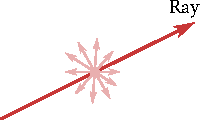
\includegraphics[scale=1]{figures/ch_16/fig_16_1.pdf}
		\caption[]{}
        % \caption[]{Oscillations of natural light occur in the most diverse directions perpendicular to a ray (unpolarized light).}
		\label{fig:16_1}
	\end{center}
	\vspace{-0.8cm}
\end{figure}

In natural light, the oscillations in different directions follow one another rapidly and without any order.
Light in which the direction of the oscillations has been brought into order in some way or other is called \textbf{polarized}.
If the oscillations of the light vector occur only in a single plane passing through a ray, the light is called \textbf{plane} (or \textbf{linearly}) \textbf{polarized}.
The order may consist in that the vector $\vec{E}$ rotates about a ray while simultaneously pulsating in magnitude.
The result is that the tip of the vector $\vec{E}$ describes an ellipse.
Such light is called \textbf{elliptically polarized}.
If the tip of the vector $\vec{E}$ describes a circle, the light is called \textbf{circularly polarized}.

We shall deal with natural light in Chapters \ref{chap:17} and \ref{chap:18}.
For this reason, we shall display no interest in the direction of the light vector oscillations.
The ways of obtaining polarized light and its properties are considered in Chapter \ref{chap:19}.

\section{Representation of Harmonic Functions Using Exponents}\label{sec:16_2}

Let us form the sum of two complex numbers $z_1 = x_1 + i y_1$ and $z_2 = x_2 + i y_2$:
\begin{equation}\label{eq:16_11}
    z = z_1 + z_2 = (x_1 + i y_1) + (x_2 + i y_2) = (x_1 + x_2) + i (y_1 + y_2).
\end{equation}

\noindent
It can be seen from \eqn{16_11} that the real part of the sum of complex numbers equals the sum of the real parts of the addends:
\begin{equation}\label{eq:16_12}
    \Re\bracet{(z_1 + z_2)} = \Re\bracet{z_1} + \Re\bracet{z_2}.
\end{equation}

Let us assume that a complex number is a function of a certain parameter, for example, of the time $t$:
\begin{equation*}
    z(t) = x(t) + i y(t).
\end{equation*}

\noindent
Differentiating this function with respect to $t$, we get
\begin{equation*}
    \diff{z}{t} = \diff{x}{t} + i \diff{y}{t}.
\end{equation*}

\noindent
It thus follows that the real part of the derivative of $z$ with respect to $t$ equals the derivative of the real part of $z$ with respect to $t$:
\begin{equation}\label{eq:16_13}
    \Re\bracet{\diff{z}{t}} = \diff{}{t}\Re\bracet{z}.
\end{equation}

A similar relation holds upon integration of a complex function.
Indeed,
\begin{equation*}
    \int z(t)\, \deriv{t} = \int x(t)\, \deriv{t} + i \int y(t)\, \deriv{t},
\end{equation*}

\noindent
whence it can be seen that the real part of the integral of $z(t)$ equals the integral of the real part of $z(t)$:
\begin{equation}\label{eq:16_14}
    \Re\bracet{\int z(t)\, \deriv{t}} = \int \Re\bracket{z(t)\, \deriv{t}}.
\end{equation}

It is evident that relations similar to Eqs. \eqref{eq:16_12}, \eqref{eq:16_13}, and \eqref{eq:16_14} also hold for the imaginary parts of complex functions.

It follows from the above that when the operations of addition, differentiation, and integration are performed with complex functions, and also linear combinations of these operations, the real (imaginary) part of the result coincides with the result that would be obtained when similar operations are performed with the real (imaginary) parts of the same functions\footnote{We must note that this rule cannot be applied to non-linear operations, for example, to the multiplication of functions and squaring them.}.
Using the symbol $\widetilde{L}$ to denote a linear combination of the operations listed above, we can write:
\begin{equation}\label{eq:16_15}
    \Re\bracet{\widetilde{L}(z_1, z_2, \ldots)} = \widetilde{L}(\Re\bracet{z_1}, \Re\bracet{z_2}, \ldots).
\end{equation}

The property of linear operations we have established makes it possible to use the following procedure in calculations: when performing linear operations with harmonic functions of the form $A \cos(\omega t - k_x x - k_y y - k_z z + \alpha)$, we can replace these functions with the exponents
\begin{equation}\label{eq:16_16}
    A \exp[i (\omega t - k_x x - k_y y - k_z z + \alpha)] = \hat{A} \exp[i (\omega t - k_x x - k_y y - k_z z)],
\end{equation}

\noindent
where $\hat{A} = A\,e^{i\alpha}$ is a complex number called the \textbf{complex amplitude}.
With such representation, we can add functions, differentiate them with respect to the variables $t$, $x$, $y$, $z$, and also integrate over these
variables.
In performing the calculations, we must take the real part of the result obtained.
The expediency of this procedure is explained by the fact that calculations with exponents are considerably simpler than calculations performed with trigonometric functions.

Passing over to representation \eqref{eq:16_16}, we in essence add to all functions of the kind $A \cos(\omega t - k_x x - k_y y - k_z z + \alpha)$ the addends $iA \sin(\omega t - k_x x - k_y y - k_z z + \alpha)$.
We remind our reader that we have used a similar procedure when studying forced oscillations (see Sec. 7.12 of Vol. I).

\section{Reflection and Refraction of a Plane Wave at the Interface Between Two Dielectrics}\label{sec:16_3}

Assume that a plane electromagnetic wave falls on the plane interface between two homogeneous and isotropic dielectrics.
The dielectric in which the incident wave is propagating is characterized by the permittivity $\varepsilon_1$, and the second dielectric by the permittivity $\varepsilon_2$.
We assume that the permeabilities are unity. Experiments show that in this case, apart from the plane refracted wave propagating in the second dielectric, a plane reflected wave propagating in the first dielectric is produced.

Let us determine the direction of propagation of the incident wave with the aid of the wave vector $\vec{k}$, of the reflected wave with the aid of the vector $\vec{k}'$ and, finally, of the refracted wave with the aid of the vector $\vec{k}''$.
We shall find how the directions of $\vec{k}'$ and $\vec{k}''$ are related to the direction of $\vec{k}$.
We can do this by taking advantage of the fact that the following condition must be observed at the interface between the two dielectrics:
\begin{equation}\label{eq:16_17}
    E_{1,\tau} = E_{2,\tau}.
\end{equation}

\noindent
Here $E_{1,\tau}$ and $E_{2,\tau}$ are the tangential components of the electric field strength in the first and second medium, respectively.

In \sect{2_7}, we proved \eqn{16_17} for electrostatic fields [see \eqn{2_44}].
It can easily be extended, however, to time-varying fields.
According to \eqn{9_5}, the circulation of $\vec{E}$ determined by \eqn{2_42} for varying fields must be not zero, but equal to the integral $\int(-\dot{\vec{B}})\ccdot\derivec{S}$ taken over the area of the loop shown in \fig{2_9}:
\begin{equation*}
    \oint E_l\, \deriv{l} = E_{1,x}a - E_{2,x}a + \average{E_b} 2b = - \int_{S=ab} \dot{\vec{B}} \ccdot \derivec{S}.
\end{equation*}

\noindent
Since $\dot{\vec{B}}$ is finite, in the limit transition $b\to 0$ the integral in the right-hand side vanishes, and we arrive at condition \eqref{eq:2_43}, from which follows \eqn{2_44}.

Assume that the vector $\vec{k}$ determining the direction of propagation of the incident wave is in the plane of the drawing (\fig{16_2}).
The direction of a normal to the interface will be characterized by the vector $\hatvec{n}$.
The plane in which the vectors $\vec{k}$ and $\hatvec{n}$ are is called the \textbf{plane of incidence} of the wave.
Let us take the line of intersection of the plane of incidence with the interface between the dielectrics
as the $x$-axis.
We shall direct the $y$-axis at right angles to the plane of the dielectric interface.
The $z$-axis will, therefore, be perpendicular to the plane of incidence, while the vector $\hatvec{\tau}$ will be directed along the $x$-axis
(see \fig{16_2}).

\begin{figure}[t]
	\begin{center}
		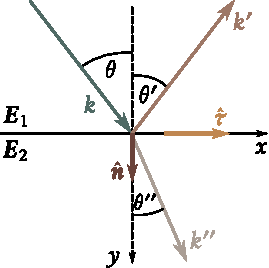
\includegraphics[scale=1]{figures/ch_16/fig_16_2.pdf}
		\caption[]{}
        % \caption[]{Propagation of incident wave ($\vec{k}$), reflecting ($\vec{k}'$) and refracting ($\vec{k}''$)} at an interface. The plane in which the vectors $\vec{k}$ and $\hatvec{n}$ are is called the plane of incidence of the wave.
		\label{fig:16_2}
	\end{center}
	\vspace{-0.8cm}
\end{figure}

It is obvious from considerations of symmetry that the vectors $\vec{k}'$ and $\vec{k}''$ can only be in the plane of incidence (the media are homogeneous and isotropic).
Indeed, assume that the vector $\vec{k}'$ has deflected from this plane ``toward us''.
There are no grounds, however, to give such a deflection priority over an equal deflection ``away from us''.
Consequently, the only possible direction of $\vec{k}'$ is that in the plane of incidence. Similar reasoning also holds for the vector $\vec{k}''$.

Let us separate from a naturally falling ray a plane-polarized component in which the direction of oscillations of the vector $\vec{E}$ makes an arbitrary angle with the plane of incidence.
The oscillations of the vector $\vec{E}$ in the plane electromagnetic wave propagating in the direction of the vector $\vec{k}$ are described by the function\footnote{More exactly, the real part of this function, but we shall say simply function for brevity's sake.}
\begin{equation*}
    \vec{E} = \ab{\vec{E}}{m} \exp[i (\omega t - \vecdot{k}{r})] = \ab{\vec{E}}{m} \exp[i (\omega t - k_x x - k_y y)]
\end{equation*}

\noindent
(with our choice of the coordinate axes, the projection of the vector $\vec{k}$ onto the $z$-axis is zero, therefore, the addend $-k_zz$ is absent in the exponent).
By correspondingly choosing the beginning of reading $t$, we have made the initial phase of the wave equal zero.

The field strengths in the reflected and refracted waves are determined by similar expressions
\begin{align*}
    \vec{E}' &= \ab{\vec{E}}{m}' \exp[i (\omega t - k_x' x - k_y' y + \alpha')]\\
    \vec{E}'' &= \ab{\vec{E}}{m}'' \exp[i (\omega t - k_x'' x - k_y'' y + \alpha'')],
\end{align*}

\noindent
where $\alpha'$ and $\alpha''$ are the initial phases of the relevant waves.

The resultant field in the first medium is
\begin{align}
    \vec{E}_1 = \vec{E} + \vec{E}' = \ab{\vec{E}}{m} \exp[i (\omega t &- k_x x - k_y y + \alpha)] \nonumber\\
    &+ \ab{\vec{E}}{m}' \exp[i (\omega t - k_x' x - k_y' y + \alpha')].\label{eq:16_18}
\end{align}

\noindent
In the second medium
\begin{equation}\label{eq:16_19}
    \vec{E}_2 = \vec{E}'' = \ab{\vec{E}}{m}'' \exp[i (\omega t - k_x'' x - k_y'' y + \alpha'')].
\end{equation}

\noindent
According to \eqn{16_17}, the tangential components of \eqns{16_18}{16_19} must be the same at the interface, \ie, when $y = 0$.
We thus arrive at the expression
\begin{align}
    \ab{E}{m,$\tau$} \exp[i(\omega t - k_xx)] + \ab{E}{m,$\tau$}' &\exp[i(\omega' t - k_xx' + \alpha')] \nonumber\\
    &= \ab{E}{m,$\tau$}'' \exp[i(\omega'' t - k_xx + \alpha'')].\label{eq:16_20}
\end{align}

For condition \eqref{eq:16_20} to be observed at any $t$, all the frequencies must be the same:
\begin{equation}\label{eq:16_21}
    \omega = \omega' = \omega''.
\end{equation}

\noindent
To convince ourselves that this is true, let us write \eqn{16_20} in the form
\begin{equation*}
    a \exp(i\omega t) + b \exp(i\omega' t) = c\exp(i\omega'' t),
\end{equation*}

\noindent
where the coefficients $a$, $b$, and $c$ are independent of $t$.
The equation which we have written is equivalent to the following two:
\begin{align*}
    a \cos(\omega t) + b \cos(\omega' t) &= c \cos(\omega'' t)\\
    a \sin(\omega t) + b \sin(\omega' t) &= c \sin(\omega'' t).
\end{align*}

\noindent
The sum of two harmonic functions will also be a harmonic function only if the functions being added have the same frequencies.
The harmonic function obtained as a result of addition will have the same frequency as the summated functions.
Hence, follows \eqn{16_21}.
We have, thus, arrived at the conclusion that the frequencies of the reflected and refracted waves coincide with that of the incident wave.

For condition \eqref{eq:16_20} to be observed at any $x$, the projections of the wave vectors onto the $x$-axis must be equal:
\begin{equation}\label{eq:16_22}
    k_x = k_x' = k_x''.
\end{equation}

\noindent
The angles $\theta$, $\theta'$, and $\theta''$ shown in \fig{16_2} are called the \textbf{angle of incidence}, the \textbf{angle of reflection}, and the \textbf{angle of refraction}.
A glance at the figure shows that $k_x = k\sin\theta$, $k_x' = k'\sin\theta'$, $k_x'' =
= k''\sin\theta''$.
Equation \eqref{eq:16_22} can therefore be written in the form
\begin{equation*}
    k \sin\theta = k' \sin\theta' = k'' \sin\theta''.
\end{equation*}

\noindent
The vectors $\vec{k}$ and $\vec{k}'$ have the same magnitude equal to $\omega/v_1$; the magnitude of the vector $\vec{k}''$ equals $w/v_2$.
Hence,
\begin{equation*}
    \frac{\omega}{v_1} \sin\theta = \frac{\omega}{v_1} \sin\theta' = \frac{\omega}{v_2} \sin\theta''.
\end{equation*}

\noindent
It thus follows that
\begin{align}
    \theta' &= \theta, \label{eq:16_23}\\
    \frac{\sin\theta}{\sin\theta''} &= \frac{v_1}{v_2} = n_{12}. \label{eq:16_24}
\end{align}

The relations we have obtained are obeyed for any plane-polarized component of a natural ray.
Hence, they also hold for a natural ray as a whole.

Equation \eqref{eq:16_23} expresses the \textbf{law of reflection of light}, according to which \textit{the reflected ray lies in one plane with the incident ray and the normal to the point of incidence; the angle of reflection equals the angle
of incidence}.

Equation \eqref{eq:16_24} expresses the \textbf{law of refraction of light}, according to which \textit{the refracted ray lies in one plane with the incident ray and the normal to the point of incidence; the ratio of the sine of the angle of
incidence to the sine of the angle of refraction is constant for given substances}.

The quantity $n_{12}$ in \eqn{16_24} is known as the \textbf{relative refractive index} of the second substance with respect to the first one.
Let us write this quantity in the form
\begin{equation}\label{eq:16_25}
    n_{12} = \frac{v_1}{v_2} = \frac{c}{v_2} \frac{v_1}{c} = \frac{c/v_2}{c/v_1} = \frac{n_2}{n_1}.
\end{equation}

\noindent
Thus, the relative refractive index of two substances equals the ratio of their absolute refractive indices.

Substituting the ratio $n_2/n_1$ for $n_{12}$ in \eqn{16_24}, we can write the law of refraction in the form
\begin{equation}\label{eq:16_26}
    n_1 \sin\theta = n_2 \sin\theta''.
\end{equation}

\noindent
Inspection of this equation shows that when light passes from an optically denser medium to an optically less dense one, the rays move away from a normal to the interface of the media.
An increase in the angle of incidence $\theta$ is attended by a more rapid growth in the angle of refraction $\theta''$, and when the angle $\theta$ reaches the value
\begin{equation}\label{eq:16_27}
    \ab{\theta}{cr} = \arcsin n_{12},
\end{equation}

\noindent
the angle $\theta''$ becomes equal to $\pi/2$.
The angle determined by \eqn{16_27} is called the \textbf{critical angle}.

The energy carried by an incident ray is distributed between the reflected and the refracted rays.
As the angle of incidence grows, the intensity of the reflected ray increases, while that of the refracted ray diminishes and vanishes at the critical angle.
At angles of incidence within the limits from $\ab{\theta}{cr}$ to $\pi/2$, the light wave penetrates into the second medium to a distance of the order of a wavelength $\lambda$ and then returns to the first medium.
This phenomenon is called \textbf{total internal reflection}.

Let us find the relations between the amplitudes and phases of the incident, reflected, and refracted waves.
For simplicity, we shall limit ourselves to the normal incidence of a wave onto the interface between dielectrics (we remind our reader that the dielectrics are assumed to be homogeneous and isotropic).
Assume that the oscillations of the vector $\vec{E}$ in the falling wave occur along the direction which we shall take as the $x$-axis.
It follows from considerations of symmetry that the oscillations of the vectors $\vec{E}'$ and $\vec{E}''$ also occur along the $x$-axis.
In the given case, the unit vector $\hatvec{\tau}$ coincides with the unit vector $\vecuni{x}$.
Therefore, the condition of continuity of the tangential component of the electric field strength has the form
\begin{equation}\label{eq:16_28}
    E_x + E_x' = E_x''.
\end{equation}

Expression \eqref{eq:16_8} obtained for the amplitude values of $E$ and $H$ also holds for their instantaneous values: $H \propto nE$.
It thus follows that the instantaneous value of the energy flux density is proportional to $nE^2$.
Thus, the law of energy conservation leads to the equation
\begin{equation}\label{eq:16_29}
    n_1 E_x^2 = n_1 E_x'^2 + n_2 E_x''^2.
\end{equation}

\noindent
We must note that the quantities $E_x$, $E_x'$ and $E_x''$ in \eqns{16_28}{16_29} are the instantaneous values of the projections.

Introducing $E_x''-E_x$ into \eqn{16_29} instead of $E_x'$ [see \eqn{16_28}], it is easy to see that
\begin{equation}\label{eq:16_30}
    E_x'' = \parenthesis{\frac{2 n_1}{(n_1 + n_2)}} E_x.
\end{equation}

\noindent
Using this value of $E_x''$ in \eqn{16_28}, we find that
\begin{equation}\label{eq:16_31}
    E_x' = \parenthesis{\frac{n_1 - n_2}{n_1 + n_2}} E_x.
\end{equation}

Examination of \eqn{16_30} shows that the projections of the vectors $\vec{E}$ and $\vec{E}''$ have identical signs at each moment of time.
Hence, we conclude that the oscillations in the incident wave and in the one passing into the second medium occur at the interface in the same phase---when a wave passes through the interface there is no jump in the phase.

It can be seen from \eqn{16_31} that when $n_2 < n_1$, the sign of $E_x'$ coincides with that of $E_x$.
This signifies that the oscillations in the incident and reflected waves occur at the interface in the same phase---the phase of a wave does not change upon reflection.
If $n_2 > n_1$, then the sign of $E_x'$ is opposite to that of $E_x$, the oscillations in the incident and reflected waves occur at the interface in counterphase---the phase of the wave changes in a jump by $\pi$ upon reflection.
The result obtained also holds upon the inclined falling of a wave at the interface between two transparent media.

Thus, when a light wave is reflected from an interface between an optically less dense medium and an optically denser one (when $n_1 < n_2$), the phase of oscillations of the light vector changes by $\pi$.
Such a phase change does not occur upon reflection from an interface between an optically denser medium and an optically less dense one (when $n_1 > n_2$).

Equations \eqref{eq:16_30} and \eqref{eq:16_31} have been obtained for the instantaneous values of the projections of the light vectors.
Similar relations also hold for the amplitudes of the light vectors:
\begin{equation}\label{eq:16_32}
    \ab{E}{m}'' = \parenthesis{\frac{2 n_1}{(n_1 + n_2)}} \ab{E}{m},\quad \ab{E}{m}' = \absolute{\frac{n_1 - n_2}{n_1 + n_2}} \ab{E}{m}.
\end{equation}

\noindent
These relations make it possible to find the reflection coefficient $\rho$ and the transmission coefficient $\tau$ of a light wave (for normal incidence at the interface between two transparent media).
Indeed, by definition
\begin{equation*}
    \rho = \frac{I'}{I} = \frac{n_1 \ab{E}{m}'^2}{n_1 \ab{E}{m}^2},
\end{equation*}

\noindent
where $I'$ is the intensity of the reflected wave, and $I$ is the intensity of the incident one.
Using in this equation the ratio $\ab{E}{m}'/\ab{E}{m}$ obtained from \eqn{16_32}, we arrive at the formula
\begin{equation}\label{eq:16_33}
    \rho = \parenthesis{\frac{n_{12} - 1}{n_{12} + 1}}^2.
\end{equation}

\noindent
Here, $n_{12} = n_2/n_1$ is the refractive index of the second medium relative to the first one.

We get the following expression for the transmission coefficient:
\begin{equation}\label{eq:16_34}
    \tau = \frac{I''}{I} = \frac{n_2 \ab{E}{m}''^2}{n_1 \ab{E}{m}^2} = n_{12} \parenthesis{\frac{2}{n_{12} + 1}}^2.
\end{equation}

We must note that the substitution for $n_{12}$ in \eqn{16_33} of its reciprocal $n_{21} = 1/n_{12}$ does not change the value of $\rho$.
Hence, the coefficient of reflection of the interface between two given media has the same value for both directions of propagation of light.

The index of refraction for glass is close to $1.5$. Introducing $n_{12} = 1.5$ into \eqn{16_33}, we get $\rho = 0.04$.
Thus, each surface of a glass plate reflects (with incidence close to normal) about four per cent of the luminous energy falling on it.

\section{Luminous Flux}\label{sec:16_4}

A real light wave is a superposition of waves with lengths confined within the interval $\Delta{\lambda}$.
The latter is finite even for monochromatic (single-coloured) light.
In white light, $\Delta{\lambda}$ covers the entire range of electromagnetic waves perceived by the eye, \ie, it ranges from \SIrange{0.40}{0.76}{\micro\metre}.

The distribution of the energy flux by wavelengths can be characterized with the aid of the distribution function
\begin{equation}\label{eq:16_35}
    \varphi(\lambda) = \diff{\ab{\Phi}{en}}{\lambda},
\end{equation}

\noindent
where $\deriv{\ab{\Phi}{en}}$ is the energy flux falling to the wavelengths from $\lambda$ to $\lambda+\Delta{\lambda}$.
Knowing the form of function \eqref{eq:16_35}, we can calculate the energy flux transferred by waves whose lengths are within the finite interval from $\lambda_1$ to $\lambda_2$:
\begin{equation}\label{eq:16_36}
    \ab{\Phi}{en} = \int_{\lambda_1}^{\lambda_2} \varphi(\lambda)\, \deriv{\lambda}.
\end{equation}

\noindent
The action of light on the eye (the perception of light) depends quite greatly on the wavelength.
This is easy to understand if we take into account that electromagnetic waves with $\lambda$ below \SI{0.40}{\micro\metre} and above \SI{0.76}{\micro\metre} are not perceived at all by the human eye.
The sensitivity of an average normal human eye to radiation of various wavelengths can be depicted graphically by a \textbf{curve of relative spectral sensitivity} (\fig{16_3}).
The wavelength $\lambda$ is laid off along the horizontal axis, and the relative spectral sensitivity $V(\lambda)$ along the vertical one.
The eye is most sensitive to radiation of the wavelength \SI{0.555}{\micro\metre}\footnote{It is interesting to note that this wavelength is represented with the greatest intensity in solar radiation.} (the green part of the spectrum).
The function $V(\lambda)$ for this wavelength is taken equal to unity.
The luminous intensity estimated visually for other wavelengths is lower, although the energy flux is the same.
Accordingly, $V(\lambda)$ for these wavelengths is also less than unity.
The values of the function $V(\lambda)$ are inversely proportional to the values of the energy fluxes producing a visual sensation identical in intensity:
\begin{equation*}
    \frac{V(\lambda_1)}{V(\lambda_2)} = \frac{(\deriv{\ab{\Phi}{en}})_2}{(\deriv{\ab{\Phi}{en}})_1}.
\end{equation*}

\begin{figure}[t]
	\begin{center}
		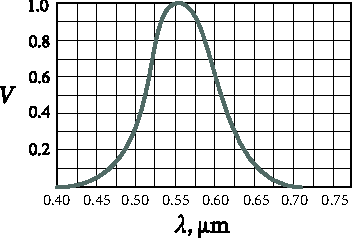
\includegraphics[scale=1]{figures/ch_16/fig_16_3.pdf}
		\caption[]{}
        % \caption[]{Curve of relative spectral sensitivity: sensitivity of an average normal human eye to radiation of various wavelengths.}
		\label{fig:16_3}
	\end{center}
	\vspace{-0.8cm}
\end{figure}

\noindent
For example, $V(\lambda) = 0.5$ signifies that for obtaining a visual sensation of the same intensity, light of the given wavelength must have a density of the energy flux twice that of light for which $V(\lambda)=1$.
Outside of the interval of visible wavelengths, the function $V(\lambda)$ is zero.

The quantity $\Phi$ called the \textbf{luminous flux} is introduced to characterize the luminous intensity with account of its ability to produce a
visual sensation.
For the interval $\deriv{\lambda}$, the luminous flux is determined as the product of the energy flux and the corresponding value of the function $V(\lambda)$:
\begin{equation}\label{eq:16_37}
    \deriv{\Phi} = V(\lambda)\, \deriv{\ab{\Phi}{en}}.
\end{equation}

\noindent
Expressing the energy flux through the function of energy distribution by wavelengths [see \eqn{16_35}], we get
\begin{equation}\label{eq:16_38}
    \deriv{\Phi} = V(\lambda) \varphi(\lambda)\, \deriv{\lambda}.
\end{equation}

\noindent
The total luminous flux is
\begin{equation}\label{eq:16_39}
    \Phi = \int_0^{\infty} V(\lambda) \varphi(\lambda)\, \deriv{\lambda}.
\end{equation}

The function $V(\lambda)$ is a dimensionless quantity.
Consequently, the dimension of luminous flux coincides with that of energy flux.
This makes it possible to define the luminous flux as the flux of luminous energy assessed according to its visual sensation.

\section{Photometric Quantities and Units}\label{sec:16_5}

Photometry is the branch of optics occupied in measuring luminous fluxes and quantities related to them.

\textbf{Luminous Intensity.}
A source of light whose dimensions may be disregarded in comparison with the distance from the place of observation to the source is called a \textbf{point source}.
In a homogeneous and isotropic medium, the wave emitted by a point source will be spherical.
Point sources of light are characterized by the luminous intensity $I$ determined as the luminous flux emitted by a source per unit solid angle:
\begin{equation}\label{eq:16_40}
    I = \diff{\Phi}{\Omega}
\end{equation}

\noindent
$\deriv{\Phi}$ is the luminous flux emitted by a source within the limits of the solid angle $\deriv{\Omega}$).

In the general case, the luminous intensity depends on the direction: $I=I(\theta,\varphi)$ (here $\theta$ and $\varphi$ are the polar and the azimuth angles in a spherical system of coordinates).
If $I$ does not depend on the direction, the light source is called \textbf{isotropic}.
For an isotropic source
\begin{equation}\label{eq:16_41}
    I = \frac{\Phi}{4\pi},
\end{equation}

\noindent
where $\Phi$ is the total luminous flux emitted by the source in all directions.

When dealing with an extended source, we can speak of the luminous intensity of an element of its surface $\deriv{S}$.
Now by $\deriv{\Phi}$ in \eqn{16_40} we must understand the luminous flux emitted by the surface
element $\deriv{S}$ within the limits of the solid angle $\deriv{\Omega}$.

The unit of luminous intensity---the candela (\si{\candela}) is one of the basic SI units.
It is defined as the luminous intensity, in the perpendicular direction, of a surface of $1/600000$ square metre of a complete radiator at the temperature of freezing platinum under a pressure of
$101325$ pascals.
By a complete radiator is meant a device having the properties of a blackbody (see Vol. III).

\textbf{Luminous Flux.}
The unit of luminous flux is the lumen (\si{\lumen}).
It equals the luminous flux emitted by an isotropic source with a luminous intensity of $1$ candela within a solid angle of one steradian:
\begin{equation}\label{eq:16_42}
    \SI{1}{\lumen} = \SI{1}{\candela} \cdot \SI{1}{\steradian}.
\end{equation}

It has been established experimentally that an energy flux of \SI{0.0016}{\watt} corresponds to a luminous flux of \SI{1}{\lumen} formed by radiation
having a wavelength of $\lambda = \SI{0.555}{\micro\metre}$.
The energy flux
\begin{equation}\label{eq:16_43}
    \ab{\Phi}{en} = \frac{0.0016}{V(\lambda)} \si{\watt},
\end{equation}

\noindent
corresponds to a luminous flux of \SI{1}{\lumen} formed by radiation of a different wavelength.

\textbf{Illuminance.}
The degree of illumination of a surface by the light falling on it is characterized by the quantity
\begin{equation}\label{eq:16_44}
    E = \diff{\ab{\Phi}{inc}}{S},
\end{equation}

\noindent
known as the \textbf{illuminance} or \textbf{illumination} ($\deriv{\ab{\Phi}{inc}}$ is the luminous flux incident on the surface element $\deriv{S}$).

The unit of illuminance is the lux (\si{\lux}) equal to the illuminance produced by a flux of \SI{1}{\lumen} uniformly distributed over a surface
having an area of \SI{1}{\metre\squared}:
\begin{equation}\label{eq:16_45}
    \SI{1}{\lux} = \SI{1}{\lumen} : \SI{1}{\metre\squared}.
\end{equation}

The illuminance $E$ produced by a point source can be expressed through the luminous intensity $I$, the distance $r$ from the surface to the source, and the angle $\alpha$ between a normal to the surface $\hatvec{n}$ and the direction to the source.
The flux incident on the area $\deriv{S}$ (\fig{16_4}) is $\deriv{\ab{\Phi}{inc}}=I\, \deriv{\Omega}$ and it is confined within the solid angle $\deriv{\Omega}$ subtended by $\deriv{S}$.
The angle $\deriv{\Omega}$ is $\deriv{S}\cos\alpha/r^2$.
Hence, $\deriv{\ab{\Phi}{inc}}=I\,\deriv{S} \cos\alpha/r^2$.
Dividing this flux by $\deriv{S}$, we get
\begin{equation}\label{eq:16_46}
    E = \frac{I \cos\alpha}{r^2}.
\end{equation}

\begin{figure}[t]
	\begin{center}
		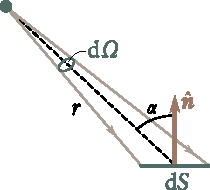
\includegraphics[scale=1]{figures/ch_16/fig_16_4.pdf}
		\caption[]{}
        % \caption[]{Incident flux $\deriv{\ab{\Phi}{inc}}$ on area $\deriv{S}$ confined by the solid angle $\deriv{\Omega}$.}
		\label{fig:16_4}
	\end{center}
	\vspace{-0.8cm}
\end{figure}

\textbf{Luminous Emittance.}
An extended source of light can be characterized by the luminous emittance $M$ of its various sections, by which is meant the luminous flux emitted outward
by unit area in all directions (within the limits of values of $\theta$ from $0$ to $\pi/2$, where $\theta$ is the angle made by the given direction with an external normal to the surface):
\begin{equation}\label{eq:16_47}
    M = \diff{\ab{\Phi}{em}}{S}
\end{equation}

\noindent
($\deriv{\ab{\Phi}{em}}$ is the flux emitted outward in all directions by the surface elements $\deriv{S}$ of the source).

Luminous emittance may appear as a result of a surface reflecting the light falling on it.
Here, by $\deriv{\ab{\Phi}{em}}$ in \eqn{16_47}, we must understand the flux reflected by the surface element $\deriv{S}$ in all directions.

The unit of luminous emittance is the lumen per square metre (\si{\lumen\per\metre\squared}).

\textbf{Luminance.}
Luminous emittance characterizes radiation (or reflection) of light by a given place of a surface in all directions.
The radiation (reflection) of light in a given direction is characterized by the luminance $L$.
The direction can be given by the polar angle $\theta$ (measured from the outward normal $\hatvec{n}$ to the emitting surface area $\Delta{S}$) and the azimuth angle $\varphi$.
Luminance is defined as the ratio of the luminous intensity of an elementary surface area $\Delta{S}$ in a given direction to the projection of the area $\Delta{A}$ onto a plane perpendicular to the chosen direction.

Let us consider the elementary solid angle $\deriv{\Omega}$ subtended by the luminous area $\deriv{S}$ and oriented in the direction $(\theta, \varphi)$ (\fig{16_5}).
The luminous intensity of area $\Delta{S}$ in the given direction, according to \eqn{16_40}, is $I = \diffin{\Phi}{\Omega}$, where $\deriv{\Phi}$ is the luminous flux propagating within the limits of the angle $\deriv{\Omega}$.
The projection of $\Delta{S}$ onto a plane normal to the direction $(\theta, \varphi)$ (in \fig{16_5} the trace of this plane is depicted by a dash line) is $\Delta{S}\cos\theta$.
Hence, the luminance is
\begin{equation}\label{eq:16_48}
    L = \frac{\deriv{\Phi}}{\deriv{\Omega} \Delta{S} \cos\theta}.
\end{equation}

\begin{figure}[t]
	\begin{center}
		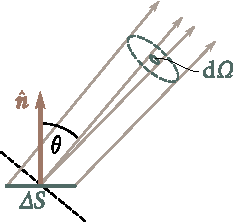
\includegraphics[scale=1]{figures/ch_16/fig_16_5.pdf}
		\caption[]{}
        % \caption[]{Elementary solid angle $\deriv{\Omega}$ subtended by the luminous area $\Delta{S}$ and oriented in the direction $(\theta,\varphi)$.}
		\label{fig:16_5}
	\end{center}
	\vspace{-0.8cm}
\end{figure}

In the general case, the luminance differs for different directions: $L=L(\theta,\varphi)$.
Like the luminous emittance, the luminance can be used to characterize a surface that reflects the light falling on it.

In accordance with \eqn{16_48}, the flux emitted by the area $\Delta{S}$ within the limits of the solid angle $\deriv{\Omega}$ in the direction determined
by $\theta$ and $\varphi$ is
\begin{equation}\label{eq:16_49}
    \deriv{\Phi} = L(\theta,\varphi)\, \deriv{\Omega} \Delta{S} \cos\theta.
\end{equation}

A source whose luminance is identical in all directions ($L = \text{constant}$) is called a \textbf{Lambertian source} (obeying Lambert's law) or a cosine source (the flux emitted by a surface element of such a source is proportional to $\cos\theta$).
Only a blackbody strictly observes Lambert's law.

The luminous emittance $M$ and luminance $L$ of a Lambertian source are related by a simple expression.
To find it, let us introduce $\deriv{\Omega}= \sin\theta\,\deriv{\theta}\,\deriv{\varphi}$ into \eqn{16_49} and integrate the expression obtained with respect to $\varphi$ within the limits from $0$ to $2\pi$ and with respect to $\theta$ from $0$ to $\pi/2$, taking into account that $L=\text{constant}$.
As a result, we shall find the total light flux emitted by surface element $\Delta{S}$ of a Lambertian source outward in all directions:
\begin{equation*}
    \Delta{\ab{\Phi}{em}} = L \Delta{S} \int_0^{2\pi} \deriv{\varphi} \int_0^{\pi/2} \sin\theta \cos\theta\, \deriv{\theta} = \pi L \Delta{S}.
\end{equation*}

\noindent
We get the luminous emittance by dividing this flux by $\Delta{S}$.
Thus, for a Lambertian source, we have
\begin{equation}\label{eq:16_50}
    M = \pi L.
\end{equation}

The unit of luminance is the candela per square metre (\si{\candela\per\metre\squared}).
A uniformly luminous plane surface has a luminance of \SI{1}{\candela\per\metre\squared} in a direction normal to it if in this direction the luminous intensity of one square metre of surface is one candela.

\section{Geometrical Optics}\label{sec:16_6}

The lengths of light waves perceived by the human eye are very small (of the order of \SI{e-7}{\metre}).
For this reason, the propagation of visible light in a first approximation can be considered without giving attention to its wave nature and assuming that light propagates along lines called \textbf{rays}.
In the limiting case corresponding to $\lambda\to 0$, the laws of optics can be formulated using the language of geometry.

Accordingly, the branch of optics in which the finiteness of the wavelengths is disregarded is known as \textbf{geometrical optics}.
Another name for it is \textbf{ray optics}.

Geometrical optics is based on four laws: (1) the law of propagation of light along a straight line; (2) the law of independence of light rays; (3) the law of light reflection; and (4) the law of refraction.

The \textbf{law of straight-line propagation} states that \textit{in a homogeneous medium light propagates in a straight line}.
This law is approximate---when light passes through very small openings, deviations from a straight line
are observed that increase with a diminishing size of the opening.

The \textbf{law of independence of light rays} states
that \textit{rays do not disturb one another when they intersect}.
The intersection of rays does not hinder each of them from propagating independently of the others. This law holds only at not too great luminous intensities.
At intensities reached with the aid of lasers, the independence of light rays stops being observed.

The laws of reflection and refraction of light were formulated in \sect{16_3} [see \eqns{16_23}{16_24} and the text following them].

Geometrical optics can be based on the principle established by the French mathematician Pierre de Fermat (1601-1665).
It underlies the laws of straight-line propagation, reflection, and refraction of light. As formulated by Fermat himself, this principle states that \textit{any light ray will travel between two end points along a line requiring the minimum transit time}.

Light needs the time $\deriv{t} = \deriv{s}/v$, where $v$ is the speed of light at the given point of the medium, to cover the distance $\deriv{s}$ (\fig{16_6}).
Replacing $v$ with $c/n$ [see \eqn{16_2}], we find that $\deriv{t}=(1/c)n\,\deriv{s}$.
Consequently, the time $\tau$ spent by light in covering the distance from point $1$ to point $2$ is
\begin{equation}\label{eq:16_51}
    \tau = \frac{1}{c} \int_1^2 n\, \deriv{s}.
\end{equation}

% \begin{figure}[t]
% 	\begin{center}
% 		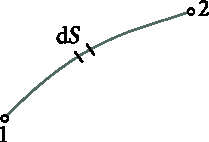
\includegraphics[scale=1]{figures/ch_16/fig_16_6.pdf}
% 		\caption[]{}
%         % \caption[]{Light ray travelling from point 1 to point 2, taking a time $\deriv{t}$ to cover a distance $\deriv{s}$ at speed $v$.}
% 		\label{fig:16_6}
% 	\end{center}
% 	\vspace{-0.8cm}
% \end{figure}
\begin{figure}[t]
	\begin{minipage}[t]{0.48\linewidth}
		\begin{center}
			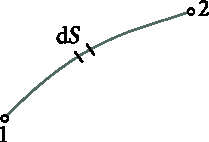
\includegraphics[scale=1]{figures/ch_16/fig_16_6.pdf}
			\caption[]{}
            % \caption[]{Light ray travelling from point 1 to point 2, taking a time $\deriv{t}$ to cover a distance $\deriv{s}$ at speed $v$.}
			\label{fig:16_6}
		\end{center}
	\end{minipage}
	\hfill{ }%space{-0.05cm}
	\begin{minipage}[t]{0.48\linewidth}
		\begin{center}
			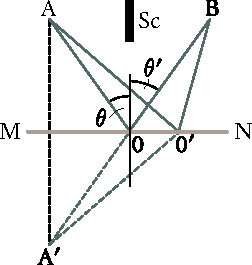
\includegraphics[scale=1]{figures/ch_16/fig_16_7.pdf}
            \caption[]{}
			% \caption[]{Reflection and refraction of light using Fermat's principle.}
			\label{fig:16_7}
		\end{center}
	\end{minipage}
\vspace{-0.4cm}
\end{figure}

The quantity
\begin{equation}\label{eq:16_52}
    L = \int_1^2 n\, \deriv{s}
\end{equation}

\noindent
having the dimension of length is called the \textbf{optical path}.
In a homogeneous medium, the optical path equals the product of the geometrical path $s$ and the index of refraction $n$ of the medium:
\begin{equation}\label{eq:16_53}
    L = ns.
\end{equation}

According to \eqns{16_51}{16_52}, we have
\begin{equation}\label{eq:16_54}
    \tau = \frac{L}{c}.
\end{equation}

\noindent
The proportionality of the time $\tau$ of covering a path to the optical path $L$ makes it possible to word Fermat's principle as follows: \textit{light travels along a path whose optical length is minimum}.
More exactly, the optical path must be extremal, \ie, either minimum or maximum, or stationary---identical for all possible paths.
In the last case, all the paths of light between two points are \textbf{tautochronous} (requiring the same time for covering them).

The reversibility of light rays ensues from Fermat's principle.
Indeed, the optical path that is minimum when light travels from point $1$ to point $2$ is also minimum when light travels in the opposite direction.
Consequently, a ray emitted toward another one that has travelled from point $1$ to point $2$ will cover the same path, but in the opposite direction.

Let us use Fermat's principle to obtain the laws of reflection and refraction of light.
Assume that a light ray reaches point B from point A after being reflected from surface MN (\fig{16_7}, the straight path from A to B is blocked by opaque screen Sc).
The medium in which the ray travels is homogeneous.
Therefore, the minimality of the optical length consists in the minimality of its geometrical length.
The geometrical length of an arbitrarily taken path is $\text{A}0'\text{B}=\text{A}'0'\text{B}$ (auxiliary point A$'$ is a mirror image of point A).
A glance at the figure shows that the path of the ray reflected at point $0$ will be the shortest.
At this point the angle of reflection equals the angle of incidence.
We must note that when point $0'$ moves away from point $0$, the geometrical path grows unlimitedly so that in the given case we have only one extreme---a minimum.

% \begin{figure}[t]
% 	\begin{center}
% 		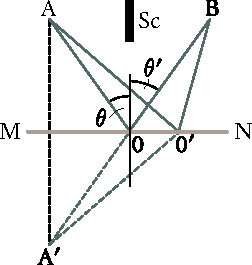
\includegraphics[scale=1]{figures/ch_16/fig_16_7.pdf}
% 		\caption[]{}
%         % \caption[]{Reflection and refraction of light using Fermat's principle.}
% 		\label{fig:16_7}
% 	\end{center}
% 	\vspace{-0.8cm}
% \end{figure}

Now let us find the point at which a ray travelling from A to B must be refracted for the optical path to be extremal (\fig{16_8}).
The optical path for an arbitrary ray is
\begin{equation*}
    L = n_1 s_1 + n_2 s_2 + n_1 \sqrt{a_1^2 + x^2} + n_2 \sqrt{a_2^2 + (b - x)^2}.
\end{equation*}

\noindent
To find the extreme value, let us differentiate $L$ with respect to $x$ and equate the derivative to zero:
\begin{equation*}
    \diff{L}{x} = \frac{n_1 x}{\sqrt{a_1^2 + x^2}} - \frac{n_2 (b - x)}{\sqrt{a_2^2 + (b - x)^2}} = n_1 \frac{x}{s_1} - n_2 \frac{(b-x)}{s_2} = 0.
\end{equation*}

\noindent
The factors of $n_1$ and $n_2$ equal $\sin\theta$ and $\sin\theta''$, respectively.
We, thus, get the relation
\begin{equation*}
    n_1 \sin\theta = n_2 \sin\theta'',
\end{equation*}

\noindent
expressing the law of refraction [see \eqn{16_26}].

Let us consider reflection from the inner surface of an ellipsoid of revolution (\fig{16_9}; $F_1$ and $F_2$ are the foci of the ellipsoid).
According to the definition of an ellipse, the paths $F_10F_2$, $F_10'F_2$, $F_10''F_2$, etc. are identical in length.
Hence, all the rays leaving focus $F_1$ and arriving after reflection at focus $F_2$ are tautochronous.
In this case, the optical path is stationary.
If we replace the surface of the ellipsoid with surface MM having a smaller curvature and oriented so that a ray leaving point $F_1$ arrives at point $F_2$ after being reflected from MM, then path $F_10F_1$ will be minimum.
For surface NN whose curvature is greater than that of the ellipsoid, path $F_10F_2$ will be maximum.

\begin{figure}[t]
	\begin{minipage}[t]{0.48\linewidth}
		\begin{center}
			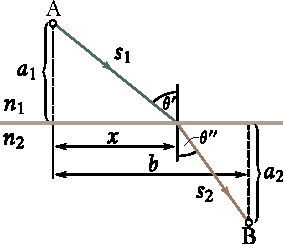
\includegraphics[scale=1]{figures/ch_16/fig_16_8.pdf}
			\caption[]{}
            % \caption[]{Ray travelling from A to B and refracted at the interface between $n_1$ and $n_2$.}
			\label{fig:16_8}
		\end{center}
	\end{minipage}
	\hfill{ }%space{-0.05cm}
	\begin{minipage}[t]{0.48\linewidth}
		\begin{center}
			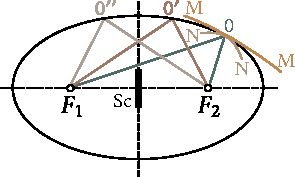
\includegraphics[scale=1]{figures/ch_16/fig_16_9.pdf}
            \caption[]{}
			% \caption[]{Reflection from the inner surface of an ellipsoid of revolution.}
			\label{fig:16_9}
		\end{center}
	\end{minipage}
\vspace{-0.4cm}
\end{figure}

The optical paths are also stationary when the rays pass through a lens (\fig{16_10}).
Ray P$0$P$'$ has the shortest path in air (where the index of refraction $n$ is virtually equal to unity) and the longest path in glass ($n\sim 1.5$).
Ray PQQ$'$P$'$ has the longest path in air, but a
shorter one in glass.
As a result, the optical paths will be the same for all the rays.
Hence, the latter are tautochronous, and the optical path is stationary.

Let us consider a wave propagating in a non-homogeneous isotropic medium along rays $1$, $2$, $3$, etc. (\fig{16_11}).
We shall consider that the non-homogeneity is sufficiently small for us to assume the index of refraction to be constant on sections of the rays of length $\lambda$.
We shall construct wave surfaces S$_1$, S$_2$, S$_3$, etc., so that the oscillations at the points of each following surface, lag in phase by $2\pi$ behind the oscillations at the points on the preceding surface.
The oscillations at points on the same ray are described by the equation $\xi=A\cos(\omega t - kr + \alpha)$ (here, $r$ is the distance measured along the ray).
The lag in phase is determined by the expression $k\Delta{r}$, where $\Delta{r}$ is the distance between adjacent surfaces.
From the condition $k\Delta{r}=2\pi$, we find that $\Delta{r}=2\pi/k=\lambda$.
The optical length of each of the paths of geometrical length $\lambda$ is $n\lambda=\lambda_0$ [see \eqn{16_5}].
According to \eqn{16_54}, the time $\tau$ during which light covers a path is proportional to the optical length of the path.
Consequently, the equality of the optical paths signifies equality of the times needed for light to travel the relevant paths.
We, thus, arrive at the conclusion that sections of rays confined between two wave surfaces have identical optical paths and are tautochronous.
In particular, the sections of the rays between wave surfaces MM and NN depicted by dash lines in \fig{16_10} are tautochronous.

\begin{figure}[t]
	\begin{minipage}[t]{0.48\linewidth}
		\begin{center}
			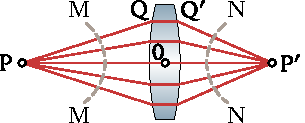
\includegraphics[scale=1]{figures/ch_16/fig_16_10.pdf}
			\caption[]{}
            % \caption[]{Stationary optical paths when light rays pass through a lens.}
			\label{fig:16_10}
		\end{center}
	\end{minipage}
	\hfill{ }%space{-0.05cm}
	\begin{minipage}[t]{0.48\linewidth}
		\begin{center}
			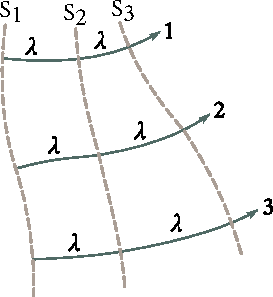
\includegraphics[scale=1]{figures/ch_16/fig_16_11.pdf}
            \caption[]{}
			% \caption[]{Wave propagating in a non-homogeneous isotropic medium along rays $1$, $2$, $3$.}
			\label{fig:16_11}
		\end{center}
	\end{minipage}
\vspace{-0.4cm}
\end{figure}

It can be seen from our treatment that the lag in phase $\delta$ appearing on the optical path $L$ is determined by the expression
\begin{equation}\label{eq:16_55}
    \delta = \frac{L}{\lambda_0} 2\pi
\end{equation}

\noindent
($\lambda_0$ is the length of a wave in a vacuum).

\section{Centered Optical System}\label{sec:16_7}

A collection of rays forms a beam.
If rays when continued intersect at one point, the beam is called homocentric.
A spherical wave surface corresponds to a homocentric beam of rays.
Figure \ref{fig:16_12}a shows a converging, and \fig{16_12}b a diverging homocentric beam.
A particular case of a homocentric beam is a beam of parallel rays; a plane light wave corresponds to it.

Any optical system transforms light beams.
If the system does not violate the homocentricity of the beams, then the rays emerging from point P intersect at one point P$'$.
This point is the \textbf{optical image} of point P. If a point of an object is depicted in the form of
a point, the image is called a \textbf{point} or a \textbf{stigmatic} one.

An image is called \textbf{real} if the light rays actually intersect at point P$'$ (see \fig{16_12}a), and virtual if the continuations of the rays in a direction opposite to the direction of propagation of the light intersect at P$'$ (see \fig{16_12}b).

\begin{figure}[t]
	\begin{center}
		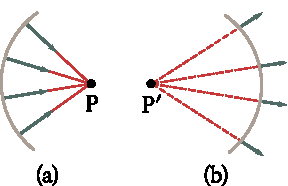
\includegraphics[scale=1]{figures/ch_16/fig_16_12.pdf}
		% \caption[]{Converging (a) and diverging (b) homocentric beam.}
        \caption[]{}
		\label{fig:16_12}
	\end{center}
	\vspace{-0.8cm}
\end{figure}

Owing to the reversibility of light rays, light source P and image P$'$ may exchange roles---a point source placed at P$'$ will have its image at P.
For this reason, P and P$'$ are called \textbf{conjugate points}.

An optical system that produces a stigmatic image which is geometrically similar to the object it depicts is called \textbf{ideal}.
With the aid of such a system, a space continuity of points P is depicted in the form of a space continuity of points P$'$.
The first continuity of points is known as the \textbf{object space}, and the second one as the \textbf{image space}.
In both spaces, points, straight lines, and planes uniquely correspond to one another.
Such a relation of two spaces is called \textbf{collinear correspondence} in geometry.

An optical system is a collection of reflecting and refracting surfaces separating optically homogeneous media from one another.
These surfaces are usually spherical or plane (a plane can be considered as a sphere of infinite radius).
More complicated surfaces such as an ellipsoid, hyperboloid or paraboloid of revolution are used much
less frequently.

An optical system formed by spherical (in particular, by plane) surfaces is called \textbf{centered} if the centres of all the surfaces are on a single straight line.
This line is called the \textbf{optical axis} of the system.
To each point P or plane S in object space there corresponds its conjugate point P$'$ or plane S$'$ in image space.
The infinite multitude of conjugate points and conjugate planes includes points and planes having special properties.
Such points and planes are called \textbf{cardinal} ones.
Among them are the \textbf{focal}, \textbf{principal}, and \textbf{nodal} points and
planes.
Setting of the cardinal points or planes completely determines the properties of an ideal centered optical system.

\textbf{Focal Planes and Focal Points of an Optical System.}
Figure \ref{fig:16_13} shows the external refracting surfaces and the optical axis of an ideal centered optical system.
Let us take plane S perpendicular to the optical axis in the object space of this system.
It follows from considerations of symmetry that plane S$'$ conjugate to S is also perpendicular to the optical axis.
Displacement of plane S relative to the system will produce a corresponding displacement of plane S$'$.
When plane S is very far, a further increase in its distance from the system will produce virtually no change in the position of plane S$'$.
This signifies that as a result of removing plane S to infinity, plane S$'$ will be in a definite extreme position F$'$. Pland F$'$ coinciding with the extreme position of plane S$'$ is called the \textbf{second} (or \textbf{hack}) \textbf{focal plane} of the optical system.
We can say briefly that the second focal plane F$'$ is defined as a plane conjugate to plane S$_{\infty}$ perpendicular to the axis of the system and at infinity in the object space.

\begin{figure}[t]
	\begin{center}
		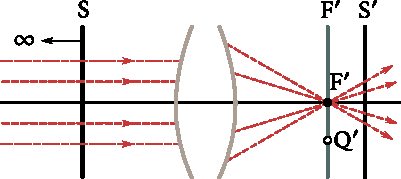
\includegraphics[scale=1]{figures/ch_16/fig_16_13.pdf}
		% \caption[]{External refracting surfaces and the optical axis of an ideal centered optical system. (Second focal point).}
        \caption[]{}
		\label{fig:16_13}
	\end{center}
	\vspace{-0.8cm}
\end{figure}

The point of intersection of the second focal plane with the optical axis is known as the \textbf{second} (or \textbf{hack}) \textbf{focal point} (\textbf{focus}) of the system.
It is also designated by the letter F$'$.
This point is conjugate to point P$_{\infty}$ on the axis of the system at infinity.
Rays emerging from P$_{\infty}$ form a beam parallel to the axis (see \fig{16_13}).
When they leave the system, these rays form a beam converging at focal point F$'$.
A parallel beam impinging on the system may leave it not in the form of a converging beam (as in \fig{16_13}), but in the form of a diverging one.
Hence, what intersects at point F$'$ will be not the
actual rays that emerge, but their extensions in the reverse direction.
Accordingly, the second focal plane will he in front (in the direction of the rays) of the system or inside it.

The rays emanating from an infinitely remote point Q$_{\infty}$, not lying on the axis of the system form a parallel beam directed at an angle to the axis of the system.
Upon emerging from the system, these rays form a beam converging at point Q$'$ belonging to the second focal plane, but not coinciding with focal point F$'$ (see point Q$'$ in \fig{16_13}).
It follows from the above that the image of an infinitely remote object will be in the focal plane.

If we remove plane S$'$ perpendicular to the axis to infinity (\fig{16_14}), its conjugate plane S will advance to its extreme position F called the \textbf{first} (or \textbf{front}) \textbf{focal plane} of the system.
We can say for short that the first focal plane F is a plane conjugate to planes S$_{\infty}'$ perpendicular to the axis of the system and at infinity in the image space.

\begin{figure}[t]
	\begin{center}
		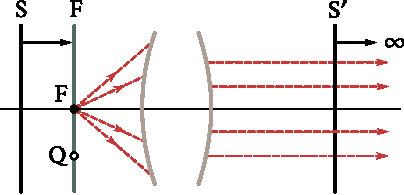
\includegraphics[scale=1]{figures/ch_16/fig_16_14.pdf}
		% \caption[]{External refracting surfaces and the optical axis of an ideal centered optical system. (First focal point).}
        \caption[]{}
		\label{fig:16_14}
	\end{center}
	\vspace{-0.8cm}
\end{figure}

The point of intersection of first focal plane F with the optical axis is called the \textbf{first} (or \textbf{front}) \textbf{focal point} (\textbf{focus}) of the system.
This point is also designated by the symbol F.
The rays emerging from focal point F form a beam of rays parallel to the axis after leaving the system. The rays emerging from point Q belonging to focal plane F (see \fig{16_14}) form a parallel beam directed at an angle to the axis of the system after passing through the latter.
It may happen that a beam which is parallel upon leaving a system is obtained when a converging beam of light falls on the system instead of a diverging one (as in \fig{16_14}).
In this case, the first focal point is either beyond the system or inside it.

\textbf{Principal Planes and Points.}
Let us consider two conjugate planes at right angles to the optical axis of the system.
Arrow $y$ (\fig{16_15}) in one of these planes will have as its image arrow $y'$ in the other plane.
It follows from axial symmetry of the system that arrows $y$ and $y'$ must be in the same plane passing through the optical axis (in the plane of the drawing).
The image $y'$ may be in the same direction as object $y$ (see \fig{16_15}a), or in the opposite direction (see \fig{16_15}b).
In the first case, the image is called \textbf{erect}, in the second---\textbf{inverted}.
Segments laid off upward from an optical axis are considered to be positive, and those laid off downward---negative.
The actual lengths of the segments are shown in drawings, \ie, the positive quantities ($-y$) and ($-y'$) for negative segments.

\begin{figure}[t]
	\begin{center}
		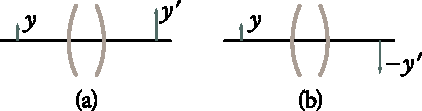
\includegraphics[scale=1]{figures/ch_16/fig_16_15.pdf}
		% \caption[]{Conjugate planes at right angles to the optical axis of the system. The image $y'$ may be in the same direction as object $y$ (a), or in the opposite direction (b).}
        \caption[]{}
		\label{fig:16_15}
	\end{center}
	\vspace{-0.8cm}
\end{figure}

The ratio of the linear dimensions of an image and an object is called the \textbf{linear} (\textbf{longitudinal}) or the \textbf{lateral magnification}.
Designating it by the symbol $M$, we can write
\begin{equation}\label{eq:16_56}
    M = \frac{y'}{y}.
\end{equation}

\noindent
The linear magnification is an algebraic quantity.
It is positive if the image is erect (the signs of $y$ and $y'$ are the same) and negative if the image is inverted (the signs of $y$ and $y'$ are opposite).

We can prove that there are two conjugate planes which reflect each other with a linear magnification of $M=+1$.
These planes are known as the \textbf{principal ones}.
The plane belonging to the object space is called the \textbf{first} (or \textbf{front}) principal plane of a system.
It is designated by the symbol H. The plane belonging to the image space is called the \textbf{second} (or \textbf{back}) \textbf{principal plane}.
Its symbol is H$'$.
The points of intersection of the principal planes with the optical axis are called the \textbf{principal points} of the system (first and second, respectively).
They are designated by the same symbols H and H$'$.
Depending on the design of a system, its principal planes and points may be either outside or inside the system.
One of the planes may be outside and the other inside a system.
Finally, both planes may be outside a system at the same side of it.

It can be seen from the definition of the principal planes that ray $1$ intersecting (actually---\fig{16_16}a, or when virtually continued inside the system---\fig{16_16}b) the first principal plane H at point Q has as its conjugate ray $1'$ that intersects (directly or upon virtual continuation) principal plane H$'$ at point Q$'$.
The latter is in the same direction and at the same distance from the axis as point Q.
This is easy to understand if we remember that Q and Q$'$ are conjugate points, and take into account that any ray passing through point Q must
have as its conjugate a ray passing through point Q$'$.

\begin{figure}[t]
	\begin{center}
		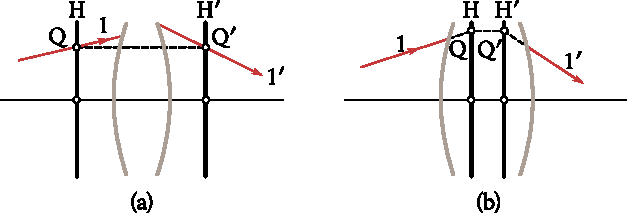
\includegraphics[scale=1]{figures/ch_16/fig_16_16h.pdf}
		% \caption[]{Conjugate points of the system intersecting principal planes.}
        \caption[]{}
		\label{fig:16_16}
	\end{center}
	\vspace{-0.7cm}
\end{figure}

\textbf{Nodal Planes and Nodal Points.}
Conjugate points N and N' lying on the optical axis and having the property that the conjugate rays passing through them (actually or when imaginarily continued inside the system) are parallel to each other are called \textbf{nodal points} or \textbf{nodes} (see rays $1$-$1'$ and $2$-$2'$ in \fig{16_17}).
Planes perpendicular to the axis and passing through the nodal points are called \textbf{nodal planes} (first and second).

The distance between the nodal points always equals that between the principal points.
When the optical properties of the media at both sides of the system are the same (\ie, $n = n'$), the nodal and principal points coincide.

\begin{figure}[t]
	\begin{center}
		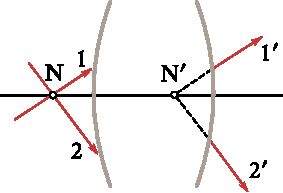
\includegraphics[scale=1]{figures/ch_16/fig_16_17.pdf}
		% \caption[]{Conjugate points N and N' lying on the optical axis.}
        \caption[]{}
		\label{fig:16_17}
	\end{center}
	\vspace{-0.8cm}
\end{figure}

\textbf{Focal Lengths and Optical Power of a System.}
The distance from first principal point H to first focal point F is called the \textbf{first focal length} $f$ of the system.
The distance from H' to F' is known as the \textbf{second focal length} $f'$.
The focal lengths $f$ and $f'$, are algebraic quantities.
They are positive if a given focal point is at the right of the relevant principal point, and negative in the opposite case.
For example, for the system shown in \fig{16_18} (see below), the second focal length $f'$ is positive, and the first focal length $f$ is negative.
The figure depicts the true length of HF, \ie, the positive quantity (-$f$) equal to the absolute value of $f$.

We can show that the following relation holds between the focal lengths $f$ and $f'$ of a centered optical system formed by spherical refracting surfaces:
\begin{equation}\label{eq:16_57}
    \frac{f}{f'} = -\frac{n}{n'},
\end{equation}

\noindent
where $n$ is the refractive index of the medium in front of the optical system, and $n'$ is the refractive index of the medium behind the system.
Examination of \eqn{16_57} shows that when the refractive indices of the media at both sides of an optical system are the same, the focal lengths differ only in their sign:
\begin{equation}\label{eq:16_58}
    f' = -f.
\end{equation}

The quantity
\begin{equation}\label{eq:16_59}
    P = \frac{n'}{f'} = - \frac{n}{f},
\end{equation}

\noindent
is known as the \textbf{optical power} of a system.
When $P$ grows, the focal length $f'$ diminishes, and, consequently, the rays are refracted by the optical system to a greater extent.
The optical power is measured in dioptres (D).
To obtain $P$ in dioptres, the focal length in \eqn{16_59} must be taken in metres.
When $P$ is positive, the second focal length $f'$ is also positive; hence, the system produces a real image of an infinitely remote point---a parallel beam of rays is transformed into a converging one.
In this case, the system is called \textbf{converging}.
When $P$ is negative, the image of an infinitely remote point will be virtual---a parallel beam of rays is transformed by the system into a diverging one. Such a system is called \textbf{diverging}.

\begin{figure}[t]
	\begin{center}
		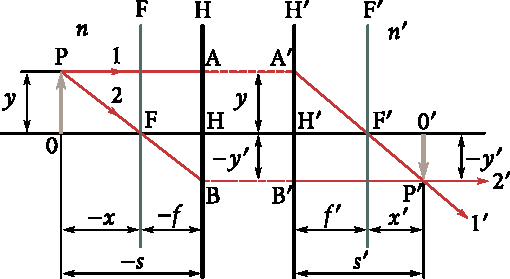
\includegraphics[scale=1]{figures/ch_16/fig_16_18.pdf}
		% \caption[]{Focal length of an optical system: the second focal length $f'$ is positive and the first focal length $f$ is negative.}
        \caption[]{}
		\label{fig:16_18}
	\end{center}
	\vspace{-0.8cm}
\end{figure}

\textbf{Formula of a System.}
We completely determine the properties of an optical system by setting its cardinal planes or points.
In particular, knowing the position of the cardinal planes, we can construct the optical image produced by a system.
Let us take segment OP perpendicular to the optical axis in the object space (\fig{16_18}, the nodal points are not shown in the figure). The position of this segment can be set either by the distance $x$ measured from point F to point $0$, or by the distances from H to $0$.
The quantities $x$ and $s$, like the focal lengths $f$ and $f'$, are algebraic ones (their magnitudes are shown in figures).

Let us draw ray $1$ parallel to the optical axis from point P.
It will intersect plane H at point A.
In accordance with the properties of principal planes, ray $1'$ conjugate to ray $1$ must pass through point A$'$ of plane H$'$ conjugate to point A.
Since ray $1$ is parallel to the optical axis, then ray $1'$ conjugate to it will pass through second focal point F$'$.
Now let us draw ray $2$ passing through the first focal point F from point P.
It will intersect plane H at point B.
Ray $2'$ conjugate to it will pass through point B$'$ of plane H$'$ conjugate to B and will be parallel to the optical axis.
Point P$'$ of intersection of rays $1'$ and $2'$
is the image of point P.
Image $0'$P$'$, like object OP, is perpendicular
to the optical axis.

The position of image $0'$P$'$ can be characterized either by the distance $x'$ from point F$'$ to point $0'$ or by the distance $s'$ from H$'$ to $0'$.
The quantities $x'$ and $s'$ are algebraic ones.
For the case shown in \fig{16_18}, they are positive.

The quantity $x'$ determining the position of the image is related to the quantity $x$ determining the position of the object and to the focal lengths $f$ and $f'$.
For the right triangles with a common apex at point F (see \fig{16_18}), we can write the relation
\begin{equation}\label{eq:16_60}
    \frac{\text{OP}}{\text{HB}} = \frac{y}{-y'} = \frac{-x}{-f}.
\end{equation}

\noindent
Similarly, for the triangles with their common apex at point F$'$, we have
\begin{equation}\label{eq:16_61}
    \frac{\text{H$'$A$'$}}{\text{O$'$P$'$}} = \frac{y}{-y'} = \frac{f'}{x'}.
\end{equation}

\noindent
Combining both relations, we find that $(-x)/(-f)=f'/x'$, whence
\begin{equation}\label{eq:16_62}
    xx' = ff'.
\end{equation}

\noindent
This equation is known as \textbf{Newton's formula}.
For the condition that $n = n'$, Newton's formula has the form
\begin{equation}\label{eq:16_63}
    xx' = -f^2
\end{equation}

\noindent
[see \eqn{16_57}].

It is easy to pass over from the formula relating the distances $x$ and $x'$ to the object and to the image from the focal points of a system to a formula establishing the relation between the distances $s$ and $s'$ from the principal points.
A glance at \fig{16_18} shows that $(-x) =
= (-s) - (-f)$ (\ie, $x=s-f$), and $x'=s'-f'$.
Introducing these expressions for $x$ and $x'$ into \eqn{16_62} and making the relevant transformations, we get
\begin{equation}\label{eq:16_64}
    \frac{f}{s} + \frac{f'}{s'} = 1.
\end{equation}

\noindent
When the condition is observed that $f'=-f$ [see \eqn{16_58}], \eqn{16_64} is simplified as follows:
\begin{equation}\label{eq:16_65}
    \frac{1}{s} - \frac{1}{s'} = \frac{1}{f}.
\end{equation}

\noindent
Equations \eqref{eq:16_62}-\eqref{eq:16_65} are equations of a centered optical system.

\section{Thin Lenses}\label{sec:16_8}

A \textbf{lens} is a very simple centered optical system.
It is a transparent (usually glass) body bounded by two spherical surfaces\footnote{There are also lenses with surfaces having a more intricate shape.} (in a particular
case one of the surfaces can be plane).
The points of intersection of the surfaces with the optical axis of a lens are called the \textbf{apices} of the refracting surfaces.
The distance between the apices is named the \textbf{thickness} of the lens.
If the lens thickness may be ignored in comparison with the smaller of the radii of curvature of the surfaces bounding a lens, the latter is called \textbf{thin}.

Calculations which we do not give here show that for a thin lens the principal planes H and H$'$ may be considered to coincide and pass through the centre $0$ of the lens (\fig{16_19}).
The following expression is obtained for the focal lengths of a thin lens:
\begin{equation}\label{eq:16_66}
    f' = -f = \parenthesis{\frac{n_0}{n-n_0}} \parenthesis{\frac{R_1R_2}{R_2-R_1}},
\end{equation}

\noindent
where $n$ is the refractive index of the lens, $n_0$ is the refractive index of the medium surrounding the lens, $R_1$ and $R_2$ are the radii of curvature of the lens surfaces.

\begin{figure}[t]
	\begin{center}
		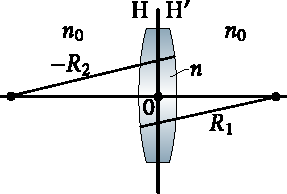
\includegraphics[scale=1]{figures/ch_16/fig_16_19.pdf}
		% \caption[]{Thin lens system: $n$ is the refractive index of the lens, $n_0$ is the refractive index of the medium surrounding the lens, $R_1$ and $R_2$ are the radii of curvature of the lens surfaces.}
        \caption[]{}
		\label{fig:16_19}
	\end{center}
	\vspace{-0.8cm}
\end{figure}

The radii of curvature must be treated as algebraic quantities: for a convex surface (\ie, when the centre of curvature is to the right of
the apex), the radius of curvature must be considered positive, and for a concave surface (\ie, when the centre of curvature is to the left of the apex) the radius must be considered
negative.
The magnitude of the radius of curvature is shown in drawings, \ie, $-R$ if $R < 0$.

If the refractive indices of the media at both sides of a thin lens are the same, then the nodal points N and N$'$ coincide with the principal points, \ie, are at the centre $0$ of the lens.
Hence, in this case, any ray passing through the centre of the lens does not change its direction.
If the refractive indices of the media before and after a lens are different, then the nodal points do not coincide with the principal points and a ray passing through the centre of the lens changes its direction.

A parallel beam of rays after passing through a lens converges at a point on the focal plane (see point Q$'$ in \fig{16_20}).
To determine the position of this point, we must continue the ray passing through the centre of the lens up to its intersection with the focal plane (see ray $0$Q$'$ shown by a dash line).
The other rays will gather at the point of intersection too.
Such a method is suitable when the optical properties of the medium at each side of a lens are identical ($n=n'$).
Otherwise, a ray passing through the centre will change its direction.
To find point Q$'$ in this case, we must know the position of the nodal points of the lens.

We must note that the optical paths laid off along the rays, beginning at wave surface SS (see \fig{16_20}) and terminating at point Q$'$
are identical and are tautochronous (see the end of \sect{16_6}).

In concluding, we must say that a lens is far from ideal optical system.
The images of objects it produces have a number of errors.
But a consideration of them is beyond the scope of the present book.

\begin{figure}[t]
	\begin{center}
		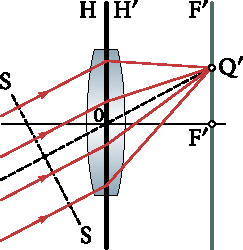
\includegraphics[scale=1]{figures/ch_16/fig_16_20.pdf}
		% \caption[]{Parallel beam of rays passign through a lens.}
        \caption[]{}
		\label{fig:16_20}
	\end{center}
	\vspace{-0.8cm}
\end{figure}

\section{Huygens' Principle}\label{sec:16_9}

In the following two chapters, we shall have to do with processes taking place behind an opaque barrier with apertures when a light wave impinges on the barrier.
In the approximation of geometrical optics, no light ought to penetrate beyond the barrier into the region of the geometrical shadow.
Actually, however, a light wave in principle propagates throughout the entire space behind the barrier and penetrates into the region of the geometrical shadow, this penetration being the more noticeable, the smaller are the dimensions of the apertures.
With a diameter of the apertures or a width of slits comparable with the length of a light wave, the approximation of geometrical optics is absolutely illegitimate.

The behaviour of light behind a barrier with an aperture can be explained qualitatively with the aid of \textbf{Huygens' principle}, named in honour of the Dutch physicist Christian Huygens (1629-1696) who discovered it.
This principle establishes the way of constructing a wavefront at the moment of time $t+\Delta{t}$ according to the known position of the wavefront at the moment $t$.
According to Huygens' principle, every point on an advancing wavefront can be considered as a source of secondary wavelets, and the envelope of these wavelets defines a new wavefront (\fig{16_21}; the medium is assumed to be non-homogeneous---the velocity of the wave in the lower part of the figure is greater than in the upper one).

\begin{figure}[t]
	\begin{minipage}[t]{0.41\linewidth}
		\begin{center}
			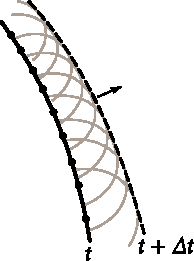
\includegraphics[scale=1]{figures/ch_16/fig_16_21.pdf}
			\caption[]{}
            % \caption[]{Huygens' principle: every point on an advancing wavefront can be considered as a source of secondary wavelets, and the envelope of these wavelets defines a new wavefront.}
			\label{fig:16_21}
		\end{center}
	\end{minipage}
	\hfill{ }%space{-0.05cm}
	\begin{minipage}[t]{0.55\linewidth}
		\begin{center}
			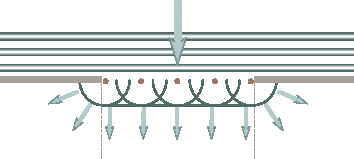
\includegraphics[scale=1]{figures/ch_16/fig_16_22.pdf}
            \caption[]{}
			% \caption[]{Huygens' diffraction: a plane barrier with an aperture is struck by a wavefront parallel to it. Every point on the portion of the wavefront bordering on the aperture is a centre of secondary wavelets which will be spherical in a homogeneous and isotropic medium.}
			\label{fig:16_22}
		\end{center}
	\end{minipage}
\vspace{-0.4cm}
\end{figure}

Assume that a plane barrier with an aperture is struck by a wavefront parallel to it (\fig{16_22}).
According to Huygens, every point on the portion of the wavefront bordering on the aperture is a centre of secondary wavelets which will be spherical in a homogeneous and isotropic medium.
Constructing the envelope of these wavelets, we shall see that the wave penetrates beyond the aperture into the region of the geometrical shadow (these regions are shown by dash lines in the figure), bending around the edges of the barrier.

Huygens' principle gives no information on the intensity of waves propagating in various directions.
This shortcoming was eliminated by the French physicist Augustin Fresnel (1788-1827).
The improved Huygens-Fresnel principle is treated in \sect{18_1}, where a physical substantiation of the principle is also given.
